\documentclass[10pt,a4paper]{article}

\usepackage[a4paper,left=0.68in,right=0.68in,top=0.62in,bottom=0.60in,headheight=13pt]{geometry}
\usepackage[T1]{fontenc}
\usepackage{lmodern}
\usepackage{microtype}
\usepackage{amsmath,amssymb,mathtools}
\usepackage{booktabs}
\usepackage{enumitem}
\usepackage{xcolor}
\usepackage{tikz}
\usetikzlibrary{arrows.meta,positioning,calc,fit,shapes.geometric}
\usepackage{pgfplots}
\pgfplotsset{compat=1.18}
\usepackage{caption}
\usepackage{graphicx}
\usepackage{fancyhdr}
\usepackage{titlesec}
\usepackage[hidelinks]{hyperref}
\usepackage{multicol}

\pagestyle{fancy}
\fancyhf{}
\lhead{Department of Computer Science and Engineering}
\rhead{Context Compression for Long-Horizon LLM Agents}
\cfoot{\thepage}

\titleformat{\section}{\large\bfseries}{\thesection.}{0.4em}{}
\titleformat{\subsection}{\normalsize\bfseries}{\thesubsection}{0.35em}{}
\setlist[itemize]{leftmargin=1.35em,itemsep=1pt,topsep=1pt}
\setlist[enumerate]{leftmargin=1.6em,itemsep=1pt,topsep=1pt}
\setlength{\parindent}{0pt}
\setlength{\parskip}{2pt}
\captionsetup{font=small,labelfont=bf}
\setlength{\abovedisplayskip}{5pt}
\setlength{\belowdisplayskip}{5pt}
\renewcommand{\topfraction}{0.9}
\renewcommand{\bottomfraction}{0.8}
\renewcommand{\textfraction}{0.07}
\renewcommand{\floatpagefraction}{0.85}

\begin{document}

% ============================================================
% TITLE PAGE
% ============================================================
\thispagestyle{empty}

\begin{center}

\vspace*{0.1cm}

\includegraphics[height=2.6cm]{"png college logo".png}

\vspace{0.35cm}

{\Large\bfseries
INDIAN INSTITUTE OF INFORMATION TECHNOLOGY\\
DESIGN AND MANUFACTURING KURNOOL\par
}

\vspace{0.25cm}

{\normalsize
Department of Computer Science and Engineering
}

\vspace{1.25cm}

{\Large\bfseries END-SEMESTER PROJECT REPORT}

\vspace{0.6cm}

\rule{0.78\textwidth}{0.6pt}

\vspace{0.65cm}

{\LARGE\bfseries
When Does Context Compression Break?\\
A Robustness Study of ACON\\
for Long-Horizon LLM Agents\par
}

\vspace{0.35cm}

{\large
\textit{Compression frequency, guideline choice and\\
held-out evaluation on AppWorld}\par
}

\vspace{0.65cm}

\rule{0.78\textwidth}{0.6pt}

\vspace{0.8cm}

{\normalsize
A report submitted in partial fulfilment of the requirements\\
for the award of the degree of\par
}

\vspace{0.35cm}

{\Large\bfseries
Bachelor of Technology
}

\vspace{0.15cm}

{\large
Computer Science and Engineering
}

\vfill

{\large\bfseries
Submitted by
}

\vspace{0.35cm}

\renewcommand{\arraystretch}{1.35}

\begin{tabular}{c l}
\textbf{123CS0006} & \textbf{Ayush Rahate}\\
\textbf{123CS0054} & \textbf{Rohit Chauhan}
\end{tabular}

\vspace{1.0cm}

{\large\bfseries
Project Supervisor
}

\vspace{0.3cm}

{\large
Dr. N. SRINIVAS NAIK
}

\vfill

\rule{0.55\textwidth}{0.4pt}

\vspace{0.35cm}

{\normalsize
Department of Computer Science and Engineering\\
Indian Institute of Information Technology Design and Manufacturing Kurnool\\
Kurnool, Andhra Pradesh -- 518008\par
}

\vspace{0.35cm}

{\normalsize
November 2026
}

\end{center}

\newpage

% ============================================================
% 1. INTRODUCTION
% ============================================================
\section{Introduction}

LLM agents solve long-horizon tasks by alternating actions and observations
over tens of steps, and every tool output and intermediate thought is appended
to the prompt. The context therefore grows without bound. This causes two
problems: inference cost grows with every step, and long, partly stale
contexts distract the model and degrade its decisions \cite{ACON}. A common
remedy is to \emph{compress} the context from time to time: a second LLM
summarises what has happened, and the agent continues from the summary.

ACON \cite{ACON} (ICML 2026) is the base paper of this project. It compresses
the history once it exceeds a threshold $T_{\mathrm{hist}}$ and long
observations once they exceed $T_{\mathrm{obs}}$, and optimises the
summariser's guideline in natural language by contrasting trajectories that
succeed without compression with ones that fail with it. In the mid-semester
report we reproduced ACON and SAC \cite{SAC}, identified three research gaps
(latency overhead, a confounded combined setting, and the lack of an intrinsic
measure of compression quality), and proposed a controlled composition pipeline
with a critical-fact retention (CFR) metric.

This semester we completed the ACON study at full scale. The results changed
the direction of the project, and this report states where and why.

\textbf{Contributions.}
\begin{enumerate}
\item A full open-weight reproduction of ACON on AppWorld (about 2,900 task runs
across train, dev and a held-out test split), including the paper's own
optimised guidelines copied verbatim from its appendix.
\item A threshold sweep on held-out tasks showing that ACON's benefit depends on
compression frequency: accuracy falls monotonically from 70.1\% at
$T_{\mathrm{hist}}=4096$ to 45.5\% at 512.
\item Controls showing that the collapse is not caused by the optimised
guideline, the summariser's size or loss of exact values, together with a
negative result for a deterministic state ledger and for two prompt-level fixes.
\item A test of ACON's combined-compression claim: the large negative
interaction it reports ($-9.5$ points) does not appear in our setting.
\item A methodological finding: on this benchmark a 56-task development split
reversed three times on the held-out split, so it is not reliable for selecting
methods.
\end{enumerate}

% ============================================================
% 2. LITERATURE REVIEW
% ============================================================
\section{Literature Review}

\textbf{Generative, prompt-level compression.} ACON \cite{ACON} uses an LLM to
rewrite the history once it exceeds a threshold $T_{\mathrm{hist}}$ and to
shorten observations longer than $T_{\mathrm{obs}}$. The compression guideline
is optimised in natural language: trajectories that succeed without
compression but fail with it are contrasted to produce feedback, and the
compressor is then distilled into smaller models. On AppWorld \cite{AppWorld}
with gpt-4.1, history compression reaches 56.5\% accuracy against 56.0\% with
no compression, and peak tokens drop by 26--54\% across three benchmarks.

\textbf{Soft, KV-level compression.} SAC \cite{SAC} selects anchor tokens from
the context, marks them with a learned embedding, and uses bidirectional
attention so that their key-value pairs absorb the whole context, without
autoencoding pretraining. On MRQA with Llama-3.2-1B at 15$\times$
compression, it reaches 54.95 in-domain F1, above EPL (51.52).

\textbf{Extractive, code-specific pruning.} SWE-Pruner \cite{SWEPruner} places
a 0.6B line-level classifier between a coding agent and its tools. The agent
writes a goal hint that conditions which lines of retrieved code are kept. On
SWE-Bench Verified it cuts tokens by 23--38\% while raising the resolve rate
by 1.2--1.4 points.

\textbf{Token pruning and RL-trained memory.} LLMLingua \cite{LLMLingua}
removes low-information tokens using a small language model. It is
task-agnostic, and in ACON's AppWorld comparison it reaches 39.3\% accuracy
for history compression. MEM1 \cite{MEM1} and MemAgent \cite{MemAgent} instead
train the agent with RL to maintain a bounded memory. MemAgent extrapolates
from an 8K window to 3.5M-token QA with under 10\% loss, but these methods
require updating the agent's weights.

\begin{table}[h]
\centering
\scriptsize
\renewcommand{\arraystretch}{1.12}
\setlength{\tabcolsep}{3pt}
\begin{tabular}{p{0.21\textwidth}cccccc}
\toprule
\textbf{Property} & \textbf{ACON} & \textbf{SAC} & \textbf{SWE-Pruner} &
\textbf{LLMLingua} & \textbf{MEM1/MemAgent} & \textbf{This work}\\
\midrule
Output form & Text & KV cache & Text lines & Text tokens & Text memory & Text\\
Agent weights frozen & Yes & Yes & Yes & Yes & No & Yes\\
History compression & Yes & No & No & Yes & Merged & Yes\\
Observation compression & Yes & No & Yes & Yes & Merged & Yes\\
Composition studied & Partly & No & No & No & No & \textbf{Yes}\\
Threshold sweep on held-out tasks & No & -- & -- & -- & -- & \textbf{Yes}\\
Intrinsic quality metric & No & No & No & No & No & \textbf{Yes (CFR)}\\
Open-weight models only & No & Yes & Yes & Yes & Yes & \textbf{Yes}\\
\bottomrule
\end{tabular}
\caption{Comparison of context-compression families. ``Partly'': ACON reports a
combined setting in an appendix ablation only. ``Merged'': one memory holds both.}
\label{tab:lit}
\end{table}

% ============================================================
% 3. IMPLEMENTATION AND RESULTS
% ============================================================
\section{Implementation and Results}

\textbf{Setup.} Table~\ref{tab:setup} lists every difference from the paper. All
models run locally through Ollama 0.20.0 on two lab workstations with one
NVIDIA RTX 2000 Ada (16\,GB) each. Both machines use identical model weights
(verified by hash). Each experiment arm runs every task once, with temperature
0; a repeated arm agreed with the original on 55 of 56 tasks, so run-to-run
variation is small compared with the effects reported.

\begin{table}[h]
\centering
\scriptsize
\renewcommand{\arraystretch}{1.12}
\begin{tabular}{p{0.2\textwidth}p{0.3\textwidth}p{0.42\textwidth}}
\toprule
\textbf{Item} & \textbf{ACON paper} & \textbf{This work}\\
\midrule
Agent & gpt-4.1 & \texttt{qwen2.5:14b} (Q4\_K\_M), served with a 16,384-token context\\
Compressor & gpt-4.1 / distilled Qwen3-14B & \texttt{qwen2.5:7b} (16,384-token context); \texttt{qwen2.5:14b} as a control\\
Guidelines & optimised with o3 & not re-optimised: the paper's own optimised prompts (Appendix D.7 history, D.10 observation) copied verbatim; the repository's unoptimised prompt (= D.5) as the baseline\\
Thresholds & $T_{\mathrm{hist}}=4096$, $T_{\mathrm{obs}}=1024$ & $T_{\mathrm{hist}}\in\{512,1024,2048,4096\}$, $T_{\mathrm{obs}}=256$\\
Agent loop & ReAct, Python REPL & same; at most 30 steps, temperature 0\\
Splits & train for optimisation, test reported & train 90 and dev 57 for development; \textbf{test\_normal 168 held out}\\
\bottomrule
\end{tabular}
\caption{Experimental setup and deviations from ACON. In September the default
4,096-token Ollama context silently truncated 32 of 38 baseline prompts; all
results here use the 16k-context variants, and the September numbers are
discarded.}
\label{tab:setup}
\end{table}

\textbf{Evaluation protocol.} All design decisions (which guideline variants
and fixes to try) were made on train and dev only. The test split was used
only for final runs of fixed configurations. Because every arm runs on the
same tasks, comparisons are paired: we report wins/losses and the exact
two-sided McNemar test, and paired bootstrap 95\% confidence intervals
(2,000 resamples) for differences in success rate. Test numbers use the 167
tasks common to all arms: task \texttt{325d6ec\_2} exhausted memory or hung in
two arms and is excluded everywhere. The research questions RQ1--RQ3 are
stated formally in Section~\ref{sec:ps}, and the interventions tested for RQ3
are described in the Proposed Solution.

\textbf{SAC reproduction and SAC$\times$ACON pilot.} The released SAC checkpoints reproduce the published MRQA scores to within
0.1 F1 (15$\times$: 54.98 / 39.25 in-domain / out-of-domain, published
54.95 / 39.26; 5$\times$: 63.70 / 47.71, published 63.63 / 47.72). In the
pilot (Llama-3.2-1B, 15$\times$, 5,000 steps), failure-gated distillation had
no effect ($-0.23$ ID F1, CI $[-0.95,+0.47]$) because the full-context teacher
was worse than the compressed student on 90.5\% of training examples.
Task-guided anchors raised F1 by about $+8.7$ ID and $+6.1$ to $+6.7$ OOD,
with or without distillation, but they condition the memory on the question, so this is a
query-aware setting rather than an improvement to SAC. Since the gaps
identified at mid-semester concern agents, the rest of the project focused on
ACON.

\textbf{RQ1: combining history and observation compression.} Table~\ref{tab:rq1} and Figure~\ref{fig:rq1}(b) use the unoptimised guideline on
all 147 train+dev tasks.
Observation compression is neutral, history compression at 512 costs 8.8
points, and combining them costs \emph{less} than history alone. The
interaction is $I=+1.4$ points (95\% CI $[-10.2,+12.2]$), so ACON's
$I=-9.5$ is not reproduced. With the paper's optimised guidelines on dev the
interaction is again positive ($+16.1$ at 512, $0.0$ at 4096). Because the
combined-compression penalty that motivated the mid-semester composition
pipeline (raw-observation buffer and schedule replay) does not occur in our
setting, we did not pursue that pipeline further.

\begin{table}[h]
\centering
\scriptsize
\renewcommand{\arraystretch}{1.12}
\setlength{\tabcolsep}{4pt}
\begin{tabular}{lcccccc}
\toprule
\textbf{Arm} ($T_{\mathrm{hist}}=512$, $T_{\mathrm{obs}}=256$) & \textbf{Solved} &
\textbf{Rate (\%)} & \textbf{Steps} & \textbf{Peak tok.} & \textbf{Agent tok./task} & \textbf{vs.\ none (McNemar)}\\
\midrule
No compression & 100/147 & 68.0 & 18.0 & 8,256 & 104.5k & --\\
History & 87/147 & 59.2 & 20.1 & 4,521 & 57.5k & $+23/-36$, $p=0.12$\\
Observation & 101/147 & 68.7 & 17.9 & 6,354 & 85.8k & $+25/-24$, $p=1.0$\\
History + observation & 90/147 & 61.2 & 19.7 & 3,108 & 53.8k & $+27/-37$, $p=0.26$\\
\midrule
\multicolumn{7}{l}{Interaction $I=\Delta(\pi_{ho})-\Delta(\pi_h)-\Delta(\pi_o)=+1.4$ points, 95\% CI $[-10.2,+12.2]$ (ACON reports $-9.5$).}\\
\bottomrule
\end{tabular}
\caption{RQ1 on train+dev (147 tasks), unoptimised guideline.}
\label{tab:rq1}
\end{table}

\begin{figure}[!htbp]
\centering
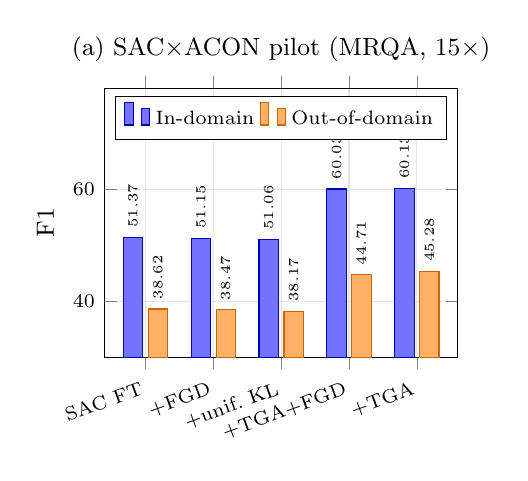
\begin{tikzpicture}
\begin{axis}[
  width=0.5\textwidth, height=5.0cm,
  ybar, bar width=7pt,
  symbolic x coords={r0,fgd,kl,tgafgd,tga},
  xtick=data,
  xticklabels={SAC FT,+FGD,+unif.\ KL,+TGA+FGD,+TGA},
  xticklabel style={font=\scriptsize, rotate=20, anchor=north east},
  ylabel={F1}, ymin=30, ymax=78,
  nodes near coords, nodes near coords style={font=\tiny, rotate=90, anchor=west},
  legend style={font=\scriptsize, at={(0.03,0.97)}, anchor=north west, legend columns=2},
  tick label style={font=\scriptsize}, label style={font=\small},
  grid=major, grid style={gray!20}, enlarge x limits=0.15,
  title={\small (a) SAC$\times$ACON pilot (MRQA, 15$\times$)},
]
\addplot[fill=blue!55, draw=blue!70!black] coordinates {(r0,51.37) (fgd,51.15) (kl,51.06) (tgafgd,60.03) (tga,60.13)};
\addlegendentry{In-domain}
\addplot[fill=orange!60, draw=orange!80!black] coordinates {(r0,38.62) (fgd,38.47) (kl,38.17) (tgafgd,44.71) (tga,45.28)};
\addlegendentry{Out-of-domain}
\end{axis}
\end{tikzpicture}
\hfill
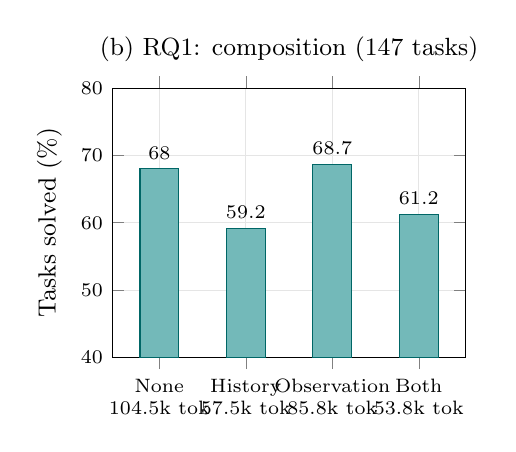
\begin{tikzpicture}
\begin{axis}[
  width=0.5\textwidth, height=5.0cm,
  ybar, bar width=14pt,
  symbolic x coords={none,hist,obs,both},
  xtick=data,
  xticklabels={{None\\104.5k tok},{History\\57.5k tok},{Observation\\85.8k tok},{Both\\53.8k tok}},
  xticklabel style={font=\scriptsize, align=center},
  ylabel={Tasks solved (\%)}, ymin=40, ymax=80,
  nodes near coords, nodes near coords style={font=\scriptsize},
  tick label style={font=\scriptsize}, label style={font=\small},
  grid=major, grid style={gray!20}, enlarge x limits=0.18,
  title={\small (b) RQ1: composition (147 tasks)},
]
\addplot[fill=teal!55, draw=teal!80!black] coordinates {(none,68.0) (hist,59.2) (obs,68.7) (both,61.2)};
\end{axis}
\end{tikzpicture}
\caption{(a) SAC pilot: failure-gated distillation (FGD) and uniform KL change
nothing; task-guided anchors (TGA) add about 9 F1 points (published SAC at
20,000 steps: 54.95 / 39.26). (b) RQ1: combining both compressors costs no more
than history compression alone, and uses the fewest agent tokens per task
(shown under each bar).}
\label{fig:rq1}
\end{figure}

\textbf{Development split: guideline, threshold and interventions.}
Table~\ref{tab:dev} shows the history-compression arms on dev (56 tasks common
to all arms). At 4096 the optimised guideline (D.7) is as good as no
compression. At 512 it collapses to 42.9\% ($p=0.0007$ against the
unoptimised guideline at the same threshold, which stays at 69.6\%). On dev the
logs pointed to a clear cause: D.7 instructs the summariser to ``delete
tool/API log output'', and its summaries mention the failures in their input
only 32\% of the time, against 87\% for the unoptimised guideline. Agents then
repeated failed attempts and called APIs that do not exist (46\% of steps
versus 36\%). Value loss was ruled out: CFR did not predict success
($r=-0.08$). Every intervention aimed at this cause helped on dev, the full
ledger fully (73.2\%, $p=0.0015$; Figure~\ref{fig:dev}).

\begin{table}[h]
\centering
\scriptsize
\renewcommand{\arraystretch}{1.12}
\setlength{\tabcolsep}{2.8pt}
\begin{tabular}{lccccc}
\toprule
\textbf{History arm (dev, 56 tasks)} & \textbf{$T_{\mathrm{hist}}$} & \textbf{Rate (\%)} &
\textbf{Summaries mention failures} & \textbf{Agent tok./task} & \textbf{vs.\ D.7@512 (McNemar)}\\
\midrule
No compression & -- & 69.6 & -- & 105.4k & $+23/-8$, $p=0.011$\\
Unoptimised guideline (D.5) & 512 & 69.6 & 87\% & 53.4k & $+17/-2$, $p=0.0007$\\
Unoptimised guideline (D.5) & 4096 & 67.9 & 51\% & 73.5k & --\\
ACON optimised (D.7) & 4096 & 73.2 & 35\% & 70.5k & $+20/-3$, $p=0.0005$\\
ACON optimised (D.7) & 512 & 42.9 & 32\% & 64.5k & --\\
\quad repeat run & 512 & 44.6 & 30\% & 61.9k & $+1/-0$\\
\midrule
D.7 + keep-failures line & 512 & 58.9 & 54\% & 53.5k & $+13/-4$, $p=0.049$\\
D.7 + keep-failures, deletion rule edited & 512 & 53.6 & 56\% & 59.9k & $+10/-4$, $p=0.18$\\
D.7 + ledger, values only & 512 & 55.4 & 35\% & 58.6k & $+13/-6$, $p=0.17$\\
D.7 + ledger, errors only & 512 & 66.1 & 43\% + ledger & 51.6k & $+16/-3$, $p=0.0044$\\
D.7 + full ledger & 512 & 73.2 & 38\% + ledger & 53.6k & $+22/-5$, $p=0.0015$\\
\bottomrule
\end{tabular}
\caption{Dev split (development only). ``Summaries mention failures'': share of
compressions whose input contained a failed step and whose LLM-written summary
mentions a failure; for ledger arms the ledger lists errors in addition.}
\label{tab:dev}
\end{table}

\begin{figure}[!htbp]
\centering
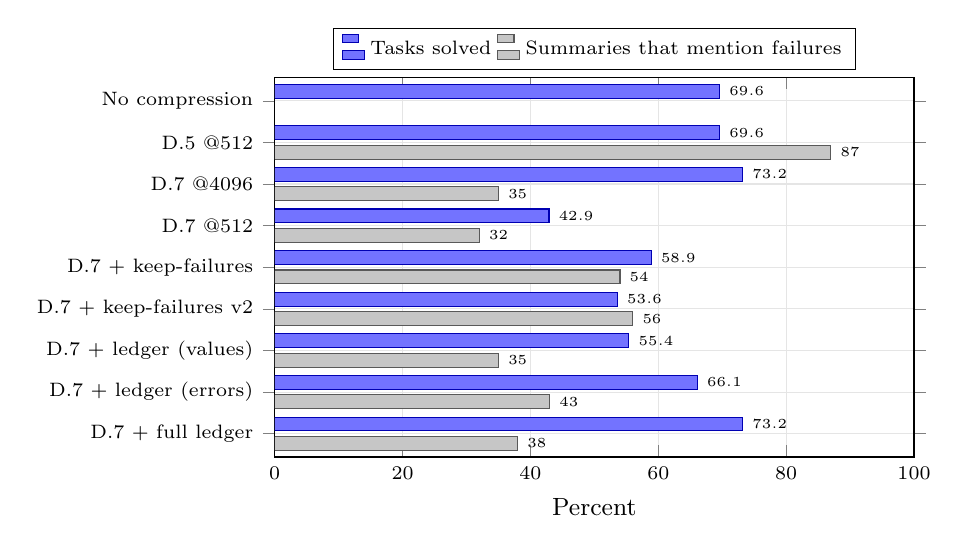
\begin{tikzpicture}
\begin{axis}[
  width=0.8\textwidth, height=6.4cm,
  xbar, bar width=5pt,
  symbolic y coords={full,err,val,kf2,kf,d7s,d74,d5s,none},
  ytick={full,err,val,kf2,kf,d7s,d74,d5s,none},
  yticklabels={D.7 + full ledger,D.7 + ledger (errors),D.7 + ledger (values),D.7 + keep-failures v2,D.7 + keep-failures,D.7 @512,D.7 @4096,D.5 @512,No compression},
  yticklabel style={font=\scriptsize},
  xmin=0, xmax=100, xlabel={Percent},
  nodes near coords, nodes near coords style={font=\tiny},
  legend style={font=\scriptsize, at={(0.5,1.02)}, anchor=south, legend columns=2},
  tick label style={font=\scriptsize}, label style={font=\small},
  grid=major, grid style={gray!20}, enlarge y limits=0.07,
  reverse legend,
]
\addplot[fill=gray!45, draw=gray!70!black] coordinates {(38,full) (43,err) (35,val) (56,kf2) (54,kf) (32,d7s) (35,d74) (87,d5s)};
\addlegendentry{Summaries that mention failures}
\addplot[fill=blue!55, draw=blue!70!black] coordinates {(73.2,full) (66.1,err) (55.4,val) (53.6,kf2) (58.9,kf) (42.9,d7s) (73.2,d74) (69.6,d5s) (69.6,none)};
\addlegendentry{Tasks solved}
\end{axis}
\end{tikzpicture}
\caption{Development split (56 tasks, $T_{\mathrm{hist}}=512$ unless stated).
On dev, success seemed to follow whether failures were kept: D.7 at 512 keeps
them least and solves least, and every fix that restores failure information
helps. Figure~\ref{fig:devtest} shows that this pattern did not hold on the
held-out tasks.}
\label{fig:dev}
\end{figure}

\textbf{RQ2 and RQ3: held-out test.} Table~\ref{tab:test} and Figure~\ref{fig:sweep} give the final results on the
held-out \texttt{test\_normal} tasks.

\begin{table}[h]
\centering
\scriptsize
\renewcommand{\arraystretch}{1.12}
\setlength{\tabcolsep}{2.2pt}
\begin{tabular}{lcccccccc}
\toprule
\textbf{Arm (test, 167 tasks)} & \textbf{Solved} & \textbf{Rate (\%)} & \textbf{Steps} &
\textbf{Step cap hit} & \textbf{Peak tok.} & \textbf{Agent tok./task} & \textbf{All-LLM tok./task} &
\textbf{Compr./task}\\
\midrule
No compression & 103 & 61.7 & 18.8 & 64 & 8,806 & 116.3k & 116.3k & 0\\
\midrule
D.7, $T_{\mathrm{hist}}=4096$ (paper) & \textbf{117} & \textbf{70.1} & 18.3 & 50 & 6,584 & 80.4k & 84.3k & 0.7\\
D.7, $T_{\mathrm{hist}}=2048$ & 111 & 66.5 & 18.6 & 56 & 5,013 & 66.0k & \textbf{71.5k} & 1.9\\
D.7, $T_{\mathrm{hist}}=1024$ & 91 & 54.5 & 21.2 & 76 & 4,237 & 64.4k & 72.8k & 4.5\\
D.7, $T_{\mathrm{hist}}=512$ & 76 & 45.5 & 22.7 & 91 & 3,768 & 63.6k & 74.8k & 9.0\\
\midrule
\multicolumn{9}{l}{\emph{Controls and fixes at $T_{\mathrm{hist}}=512$}}\\
Unoptimised guideline (D.5) & 82 & 49.1 & 21.6 & 85 & 4,096 & 62.2k & 72.7k & 8.9\\
D.7, 14B summariser & 78 & 46.7 & 22.4 & 89 & n/a & n/a & 75.0k & 9.4\\
D.7 + ledger, errors only & 81 & 48.5 & 22.7 & 86 & 4,025 & 65.0k & 79.3k & 11.4\\
D.7 + full ledger & 88 & 52.7 & 21.7 & 79 & 4,173 & 67.1k & 89.0k & 15.6\\
\bottomrule
\end{tabular}
\caption{Held-out test results. ``All-LLM tokens'' adds the summariser's input
tokens to the agent's. With a 14B summariser the agent and summariser are the
same model, so their tokens cannot be separated in our logs.}
\label{tab:test}
\end{table}

\begin{figure}[h]
\centering
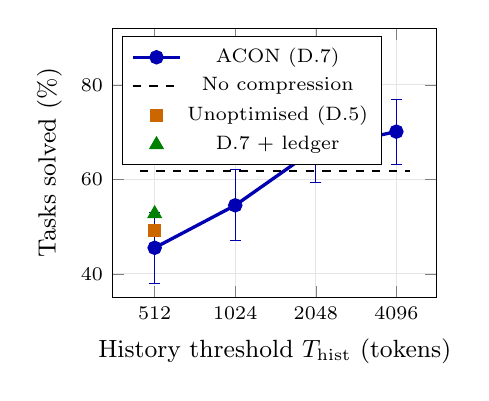
\begin{tikzpicture}
\begin{axis}[
  width=0.47\textwidth, height=5.0cm,
  xmode=log, log basis x=2,
  xtick={512,1024,2048,4096}, xticklabels={512,1024,2048,4096},
  xlabel={History threshold $T_{\mathrm{hist}}$ (tokens)},
  ylabel={Tasks solved (\%)},
  ymin=35, ymax=92,
  grid=major, grid style={gray!20},
  legend style={font=\scriptsize, at={(0.03,0.97)}, anchor=north west},
  tick label style={font=\scriptsize}, label style={font=\small},
]
\addplot[very thick, blue!70!black, mark=*,
  error bars/.cd, y dir=both, y explicit]
  coordinates {(512,45.5) +- (0,7.5) (1024,54.5) +- (0,7.5) (2048,66.5) +- (0,7.2) (4096,70.1) +- (0,6.9)};
\addlegendentry{ACON (D.7)}
\addplot[thick, dashed, black] coordinates {(450,61.7) (4600,61.7)};
\addlegendentry{No compression}
\addplot[only marks, mark=square*, orange!80!black, mark size=2.2pt] coordinates {(512,49.1)};
\addlegendentry{Unoptimised (D.5)}
\addplot[only marks, mark=triangle*, green!50!black, mark size=2.8pt] coordinates {(512,52.7)};
\addlegendentry{D.7 + ledger}
\end{axis}
\end{tikzpicture}
\hfill
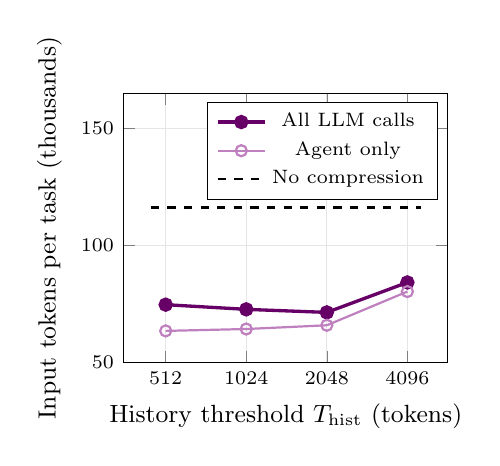
\begin{tikzpicture}
\begin{axis}[
  width=0.47\textwidth, height=5.0cm,
  xmode=log, log basis x=2,
  xtick={512,1024,2048,4096}, xticklabels={512,1024,2048,4096},
  xlabel={History threshold $T_{\mathrm{hist}}$ (tokens)},
  ylabel={Input tokens per task (thousands)},
  ymin=50, ymax=165,
  grid=major, grid style={gray!20},
  legend style={font=\scriptsize, at={(0.97,0.97)}, anchor=north east},
  tick label style={font=\scriptsize}, label style={font=\small},
]
\addplot[very thick, violet!80!black, mark=*] coordinates {(512,74.8) (1024,72.8) (2048,71.5) (4096,84.3)};
\addlegendentry{All LLM calls}
\addplot[thick, violet!50, mark=o] coordinates {(512,63.6) (1024,64.4) (2048,66.0) (4096,80.4)};
\addlegendentry{Agent only}
\addplot[thick, dashed, black] coordinates {(450,116.3) (4600,116.3)};
\addlegendentry{No compression}
\end{axis}
\end{tikzpicture}
\caption{Held-out test (167 tasks). Left: success rate against the history
threshold; bars are $\pm1.96$ binomial standard errors for each arm alone (the
paired tests in the text are more sensitive). Right: token cost. Compressing
more often than every 2048 tokens lowers accuracy without lowering the total
token cost.}
\label{fig:sweep}
\end{figure}

\begin{figure}[!htbp]
\centering
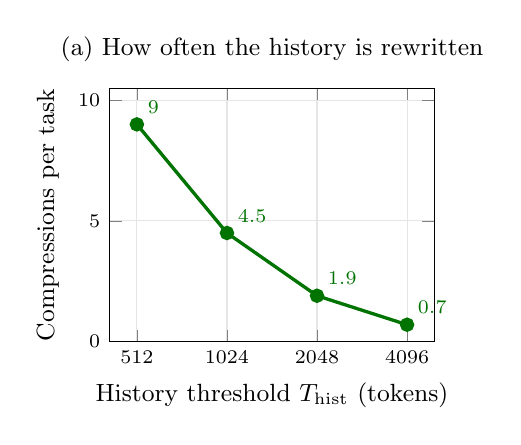
\begin{tikzpicture}
\begin{axis}[
  width=0.47\textwidth, height=4.8cm,
  xmode=log, log basis x=2,
  xtick={512,1024,2048,4096}, xticklabels={512,1024,2048,4096},
  xlabel={History threshold $T_{\mathrm{hist}}$ (tokens)},
  ylabel={Compressions per task},
  ymin=0, ymax=10.5,
  nodes near coords, nodes near coords style={font=\scriptsize, anchor=south west},
  grid=major, grid style={gray!20},
  tick label style={font=\scriptsize}, label style={font=\small},
  title={\small (a) How often the history is rewritten},
]
\addplot[very thick, green!45!black, mark=*] coordinates {(512,9.0) (1024,4.5) (2048,1.9) (4096,0.7)};
\end{axis}
\end{tikzpicture}
\hfill
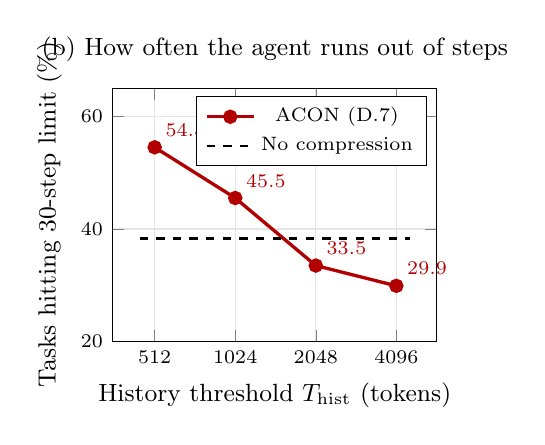
\begin{tikzpicture}
\begin{axis}[
  width=0.47\textwidth, height=4.8cm,
  xmode=log, log basis x=2,
  xtick={512,1024,2048,4096}, xticklabels={512,1024,2048,4096},
  xlabel={History threshold $T_{\mathrm{hist}}$ (tokens)},
  ylabel={Tasks hitting 30-step limit (\%)},
  ymin=20, ymax=65,
  nodes near coords, nodes near coords style={font=\scriptsize, anchor=south west},
  legend style={font=\scriptsize, at={(0.97,0.97)}, anchor=north east},
  grid=major, grid style={gray!20},
  tick label style={font=\scriptsize}, label style={font=\small},
  title={\small (b) How often the agent runs out of steps},
]
\addplot[very thick, red!70!black, mark=*] coordinates {(512,54.5) (1024,45.5) (2048,33.5) (4096,29.9)};
\addlegendentry{ACON (D.7)}
\addplot[thick, dashed, black, nodes near coords={}] coordinates {(450,38.3) (4600,38.3)};
\addlegendentry{No compression}
\end{axis}
\end{tikzpicture}
\caption{Why accuracy falls (held-out test, 167 tasks). (a) Lowering the
threshold from 4096 to 512 makes the summariser rewrite the history about 13
times as often. (b) With frequent rewrites the agent loses track of its progress
and more tasks end at the 30-step limit: 54.5\% at 512 against 29.9\% at 4096.}
\label{fig:steps}
\end{figure}

\textbf{ACON works at its own threshold.} At $T_{\mathrm{hist}}=4096$ ACON solves
70.1\% of held-out tasks against 61.7\% without compression ($+8.4$ points, CI
$[+0.0,+17.4]$) and uses 31\% fewer agent input tokens. Measured LLM time per
task is also lower (181\,s against 199\,s), so in our setting gap (a) of the
mid-semester report (compression costing time) does not appear at the paper's
threshold. It does appear at 512 (255\,s per task).

\textbf{Accuracy falls as compression becomes more frequent (RQ2).} Success
drops monotonically: 70.1, 66.5, 54.5 and 45.5\% at 4096, 2048, 1024 and 512.
The drop from 4096 to 512 is 24.6 points (CI $[+16.2,+32.9]$, McNemar
$+53/-12$, $p=2.8\times10^{-7}$), and at 512 ACON is 16.2 points \emph{worse}
than no compression (CI $[-25.7,-6.6]$). Halving the threshold to 2048 costs
little ($p=0.43$ against 4096). Below 2048 the agent needs more steps and hits
the 30-step limit more often (91 tasks at 512 against 50 at 4096;
Figure~\ref{fig:steps}).

\textbf{More frequent compression does not save tokens.} Total LLM input is
lowest at 2048 (71.5k tokens per task) and is higher at 512 (74.8k), because the
longer trajectories outweigh the shorter prompts. Thresholds below 2048 are
therefore worse on both accuracy and cost.

\textbf{The collapse is not caused by the guideline, summariser size or value
loss (RQ3).} At 512 the unoptimised guideline reaches 49.1\%, not
significantly different from D.7 ($+31/-25$, $p=0.50$), even though its
summaries mention failures 85\% of the time against 26\% for D.7 on the same
tasks. A summariser twice as large changes nothing ($46.7\%$, $p=0.89$). The
full ledger, which preserves exact values and errors, recovers 7.2 points (CI
$[-1.8,+16.2]$, $p=0.13$), and its errors-only half 3.0 points ($p=0.58$),
neither significant. The ledger also lengthens summaries, which triggers more
compressions (15.6 per task against 9.0).

\textbf{The development split misled us.} The failure-deletion mechanism, the
full ledger and the errors-only ledger all looked strong on dev
(Table~\ref{tab:dev}) and did not hold on test. On dev the unoptimised guideline
was unaffected by frequent compression (69.6\%), whereas on test it collapsed
like D.7. With 56 tasks, one task is 1.8 points, and differences of 10--15
points between arms were not stable across splits (Figure~\ref{fig:devtest}).

\begin{figure}[!htbp]
\centering
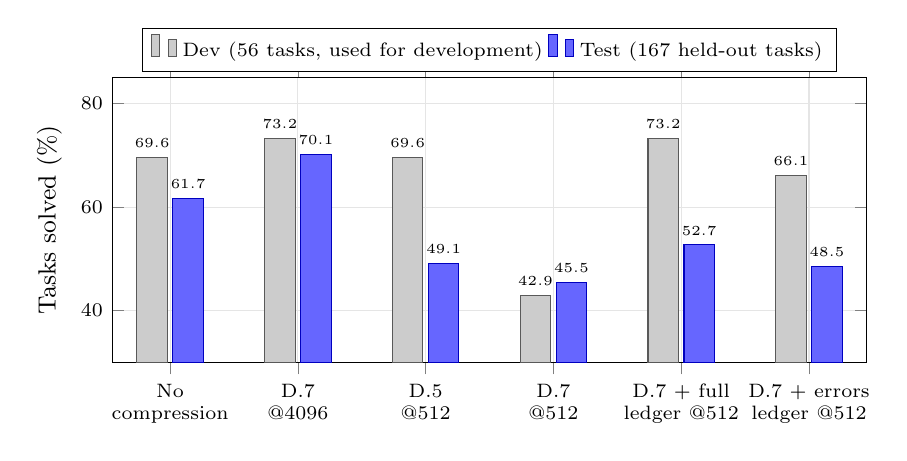
\begin{tikzpicture}
\begin{axis}[
  width=0.92\textwidth, height=5.2cm,
  ybar, bar width=11pt,
  symbolic x coords={none,d74,d5s,d7s,full,err},
  xtick=data,
  xticklabels={{No\\compression},{D.7\\@4096},{D.5\\@512},{D.7\\@512},{D.7 + full\\ledger @512},{D.7 + errors\\ledger @512}},
  xticklabel style={font=\scriptsize, align=center},
  ylabel={Tasks solved (\%)}, ymin=30, ymax=85,
  nodes near coords, nodes near coords style={font=\tiny},
  legend style={font=\scriptsize, at={(0.5,1.02)}, anchor=south, legend columns=2},
  tick label style={font=\scriptsize}, label style={font=\small},
  grid=major, grid style={gray!20}, enlarge x limits=0.09,
]
\addplot[fill=gray!40, draw=gray!70!black] coordinates {(none,69.6) (d74,73.2) (d5s,69.6) (d7s,42.9) (full,73.2) (err,66.1)};
\addlegendentry{Dev (56 tasks, used for development)}
\addplot[fill=blue!60, draw=blue!75!black] coordinates {(none,61.7) (d74,70.1) (d5s,49.1) (d7s,45.5) (full,52.7) (err,48.5)};
\addlegendentry{Test (167 held-out tasks)}
\end{axis}
\end{tikzpicture}
\caption{Development versus held-out results for the same configurations. ACON at
its own threshold and the collapse of D.7 at 512 hold on both splits; the
unoptimised guideline at 512 and both ledger fixes, which looked as good as no
compression on dev, fall to 48--53\% on test.}
\label{fig:devtest}
\end{figure}

% ============================================================
% 4. RESEARCH GAPS
% ============================================================
\section{Research Gaps}\label{sec:gaps}

The mid-semester report identified three gaps in ACON. Our full-scale results
settle them and expose new ones.

\textbf{Status of the mid-semester gaps.}
\begin{enumerate}[label=(\alph*)]
\item \textbf{Latency.} Measured directly: at the paper's threshold compression
\emph{reduces} LLM time per task (181\,s against 199\,s without compression); the
overhead appears only at low thresholds (255\,s at 512).
\item \textbf{Confounded combined setting.} The penalty it would explain does not
occur in our setting ($I=+1.4$, CI $[-10.2,+12.2]$; Table~\ref{tab:rq1}), so the
schedule-replay pipeline proposed at mid-semester was not needed.
\item \textbf{No intrinsic quality measure.} CFR was implemented and computed for
every compression call, but it does not predict task success ($r=-0.08$), so
loss of exact values is not what makes compression fail.
\end{enumerate}

\textbf{Gaps identified this semester.}
\begin{enumerate}[label=(\alph*),resume]
\item \textbf{ACON's benefit depends on compression frequency, and the paper does
not test this.} ACON reports results at one history threshold. On held-out
tasks success falls monotonically from 70.1\% at 4096 to 45.5\% at 512, below
the uncompressed agent (Figure~\ref{fig:sweep}). Lowering the threshold, the
natural way to save more tokens, costs accuracy and does not even reduce total
tokens.
\item \textbf{The guideline is not the cause.} At 512 ACON's optimised guideline
and the unoptimised one perform the same on test (45.5\% and 49.1\%,
$p=0.50$), and a summariser twice as large does not help (46.7\%). Optimising
the guideline, ACON's central contribution, therefore does not protect against
frequent compression.
\item \textbf{Small development splits mislead.} Three fixes selected on 56 dev
tasks (Table~\ref{tab:dev}) did not hold on 167 held-out tasks, and a mechanism
that was clear on dev (the optimised guideline deleting failure information)
did not explain the test results. Guideline optimisation on a small split is
exposed to the same risk.
\end{enumerate}

% ============================================================
% 5. PROBLEM STATEMENT
% ============================================================
\section{Problem Statement}\label{sec:ps}

\textbf{Agent model.} Following \cite{ACON}, a task is a POMDP
$\mathcal{E}=\langle\mathcal{S},\mathcal{A},\mathcal{O},\mathcal{T},R\rangle$.
At step $t$ an agent $M$ with frozen parameters $\theta$ acts on the (possibly
compressed) history $h'_{t-1}$ and the latest observation $o'_t$:
\begin{equation}
a_t = M\big(h'_{t-1},\,o'_t;\,\theta\big),\qquad
h_t=(o_0,a_0,o_1,a_1,\dots,o_t,a_t).
\label{eq:agent}
\end{equation}

\textbf{Compression operators and trigger.} With history compressor $f_h$
(guideline $g$), the history is rewritten at the trigger steps
\begin{equation}
\mathcal{K}(T_{\mathrm{hist}})=\big\{\,t : |h'_{t-1}\oplus(o'_t,a_t)|>T_{\mathrm{hist}}\,\big\},
\qquad
h'_t=\begin{cases} f_h(h'_{t-1}\oplus(o'_t,a_t);\,g) & t\in\mathcal{K}\\ h'_{t-1}\oplus(o'_t,a_t) & \text{otherwise}.\end{cases}
\label{eq:trigger}
\end{equation}
A lower $T_{\mathrm{hist}}$ means more frequent compression: in our runs about
0.7 compressions per task at 4096 and 9.0 at 512.

\textbf{Quantities measured.} Success $R\in\{0,1\}$ per task (AppWorld's
state-based checker), the gain over no compression
$\Delta(\pi)=\mathbb{E}[R(\pi)]-\mathbb{E}[R(\pi_\varnothing)]$, agent token cost
$C(\pi)=\sum_t(|h'_{t-1}|+|o'_t|)$, peak context
$P(\pi)=\max_t(|h'_{t-1}|+|o'_t|)$, and, for combined compression, the interaction
\begin{equation}
I=\Delta(\pi_{ho})-\Delta(\pi_h)-\Delta(\pi_o).
\label{eq:interaction}
\end{equation}
For ACON on AppWorld, $I=-9.5$ points \cite{ACON}. The critical-fact retention
rate CFR (defined in the mid-semester report) is the share of task-critical
values (tokens, IDs, numbers) present in the input of a compression that
survive verbatim in its output.

\textbf{Research questions.}
\begin{enumerate}[label=\textbf{RQ\arabic*.}]
\item Does ACON's large penalty for combining history and observation
compression ($I=-9.5$) reproduce with open-weight models?
\item How does task success depend on the compression frequency
$T_{\mathrm{hist}}$, for ACON's optimised guideline, on held-out tasks?
\item What causes the change, and can it be removed without giving up the
token savings?
\end{enumerate}

% ============================================================
% 6. PROPOSED SOLUTION
% ============================================================
\section{Proposed Solution}

To answer RQ3 we proposed and tested interventions that target the likely
causes of the collapse, each against a matched control
(Figure~\ref{fig:pipe}).

\begin{itemize}
\item \textbf{State ledger.} A deterministic extractor (Python syntax tree and
regular expressions, no LLM) that reads the raw steps being compressed and
appends a verbatim block to the summary: variables still in the REPL,
credentials seen, APIs already called with their literal arguments, APIs the
environment reported as non-existent, and the last three errors. Its two halves
(``values'' and ``errors'') can be enabled separately.
\item \textbf{Guideline edits.} D.7 plus the unoptimised guideline's line
``Include key info from errors or failed attempts to prevent repeated
mistakes'' (\emph{keep-failures}), and a second version that also removes
``tool/API log output'' from D.7's deletion rule.
\item \textbf{Controls.} The unoptimised guideline (D.5) and a 14B summariser
at the same threshold, to separate the effect of the guideline and of the
summariser's capacity from that of compression frequency.
\item \textbf{Instrumentation.} Per-request logging of prompt and completion
tokens and latency for both models, CFR for every compression call, and a
keyword test of whether each summary mentions the failures in its input.
\end{itemize}

\begin{center}
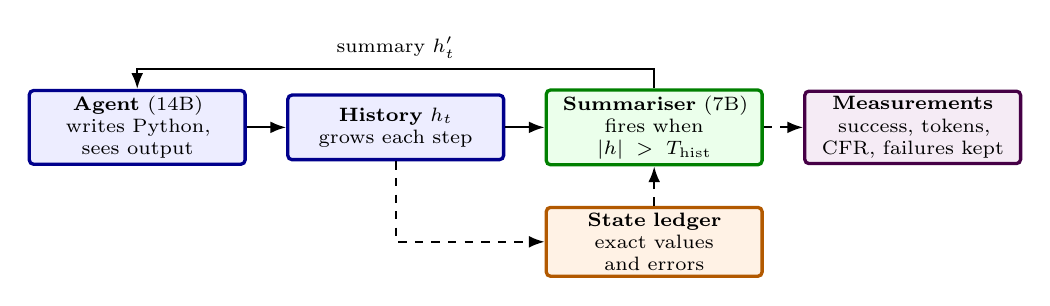
\begin{tikzpicture}[
  font=\scriptsize,
  bx/.style={draw, rounded corners=1.5pt, very thick, align=center,
    text width=2.6cm, minimum height=0.82cm, inner sep=2pt},
  arr/.style={-{Latex[length=2mm]}, line width=0.7pt},
  env/.style={bx, fill=blue!7, draw=blue!55!black},
  cmp/.style={bx, fill=green!8, draw=green!50!black},
  ctl/.style={bx, fill=orange!10, draw=orange!70!black},
  met/.style={bx, fill=violet!8, draw=violet!55!black}
]
\node[env] (ag) {\textbf{Agent} (14B)\\writes Python, sees output};
\node[env, right=5mm of ag] (h) {\textbf{History} $h_t$\\grows each step};
\node[cmp, right=5mm of h] (hc) {\textbf{Summariser} (7B)\\fires when $|h|>T_{\mathrm{hist}}$};
\node[ctl, below=5mm of hc] (led) {\textbf{State ledger}\\exact values\\and errors};
\node[met, right=5mm of hc] (m) {\textbf{Measurements}\\success, tokens,\\CFR, failures kept};
\draw[arr] (ag)--(h);
\draw[arr] (h)--(hc);
\draw[arr] (hc.north) -- ++(0,0.25) -| node[pos=0.25,above]{summary $h'_t$} (ag.north);
\draw[arr, dashed] (h.south) |- (led.west);
\draw[arr, dashed] (led.north) -- (hc.south);
\draw[arr, dashed] (hc)--(m);
\end{tikzpicture}
\end{center}
\captionof{figure}{Pipeline studied. The ledger (orange, optional) is extracted
from the raw steps without an LLM and appended to the summary.}
\label{fig:pipe}

\textbf{Outcome.} On dev, every intervention aimed at preserving failures
helped, and the full ledger restored accuracy completely (73.2\%,
Table~\ref{tab:dev}). On the held-out tasks none of them removed the collapse:
the full ledger recovered 7.2 points (CI $[-1.8,+16.2]$, $p=0.13$), the
errors-only ledger 3.0 points ($p=0.58$), the unoptimised guideline 3.6 points
($p=0.50$) and the larger summariser 1.2 points ($p=0.89$). The ledger also
lengthens each summary, which triggers more compressions (15.6 per task
against 9.0). The evidence therefore points to the \emph{number} of rewrites,
not to what a particular guideline keeps, as the factor that matters. The
solution that works in our data is operational: keep the history threshold at
2048--4096 tokens, which gives the highest accuracy (66.5--70.1\%) and the
lowest total token cost (71.5--84.3k per task) of all settings tested.

% ============================================================
% 7. FUTURE WORK
% ============================================================
\section{Future Work}

\textbf{Conclusion.} We reproduced ACON with open-weight models and evaluated
it on held-out AppWorld tasks. It improves success and cuts tokens at the
paper's threshold, but its benefit reverses when the history is compressed more
often: success falls from 70.1\% to 45.5\%, below the uncompressed agent, with no
saving in tokens. The collapse persists under the unoptimised guideline, a
larger summariser and a deterministic state ledger, and ACON's reported penalty
for combined compression does not reproduce.

\textbf{Limitations.} One benchmark (AppWorld) and one model family (Qwen2.5,
4-bit quantised); ACON's results with gpt-4.1 may be less sensitive to the
threshold, which we could not test without API access. The optimised guidelines
were copied from the paper rather than re-optimised for our models. Each
configuration was run once at temperature 0 (a repeated arm differed on 1 of 56
tasks). The failure-mention measure is a keyword test, not a human judgement.

\begin{itemize}
\item \textbf{Complete the guideline $\times$ threshold curve.} Runs of the
unoptimised guideline at 1024, 2048 and 4096 and a repeat of ACON at 512 on the
test split are in progress, to confirm that the guideline is irrelevant at every
threshold and that the collapse is stable across runs.
\item \textbf{Generalise.} Repeat the threshold sweep with a second model family
as the agent and on a second benchmark.
\item \textbf{Adaptive triggers.} Compress only at sub-task boundaries instead of
at a fixed token count, to reduce the number of rewrites while keeping the
token savings.
\item \textbf{Publication.} Write the threshold study up as a short paper
(workshop or reproducibility track), reporting the development-versus-test
reversals in full.
\end{itemize}

\begin{thebibliography}{99}

\bibitem{ACON}
M. Kang, W.-N. Chen, D. Han, H. A. Inan, L. Wutschitz, Y. Chen, R. Sim, and
S. Rajmohan,
``ACON: Optimizing Context Compression for Long-horizon LLM Agents,''
in \emph{Proc. 43rd Int. Conf. Machine Learning (ICML)}, PMLR 306, 2026.

\bibitem{SAC}
X. Liu, R. Zhao, P. Huang, X. Liu, J. Xiao, C. Xiao, T. Xiao, S. Gao, Z. Yu,
and J. Zhu,
``Autoencoding-Free Context Compression for LLMs via Contextual Semantic
Anchors,''
in \emph{Int. Conf. Learning Representations (ICLR)}, 2026.

\bibitem{SWEPruner}
Y. Wang, Y. Shi, M. Yang, R. Zhang, S. He, H. Lian, Y. Chen, S. Ye, K. Cai,
and X. Gu,
``SWE-Pruner: Self-Adaptive Context Pruning for Coding Agents,''
arXiv:2601.16746, 2026.

\bibitem{LLMLingua}
H. Jiang, Q. Wu, C.-Y. Lin, Y. Yang, and L. Qiu,
``LLMLingua: Compressing Prompts for Accelerated Inference of Large Language
Models,''
in \emph{Proc. EMNLP}, pp. 13358--13376, 2023.

\bibitem{MEM1}
Z. Zhou, A. Qu, Z. Wu, S. Kim, A. Prakash, D. Rus, J. Zhao, B. K. H. Low, and
P. P. Liang,
``MEM1: Learning to Synergize Memory and Reasoning for Efficient Long-Horizon
Agents,''
arXiv:2506.15841, 2025.

\bibitem{MemAgent}
H. Yu, T. Chen, J. Feng, J. Chen, W. Dai, Q. Yu, Y.-Q. Zhang, W.-Y. Ma, J. Liu,
M. Wang, and H. Zhou,
``MemAgent: Reshaping Long-Context LLM with Multi-Conv RL-based Memory Agent,''
in \emph{Int. Conf. Learning Representations (ICLR)}, 2026.

\bibitem{AppWorld}
H. Trivedi, T. Khot, M. Hartmann, R. Manku, V. Dong, E. Li, S. Gupta,
A. Sabharwal, and N. Balasubramanian,
``AppWorld: A Controllable World of Apps and People for Benchmarking
Interactive Coding Agents,''
in \emph{Proc. ACL}, pp. 16022--16076, 2024.

\end{thebibliography}

\end{document}
